The electroweak process \Wgstar contributes as background to the Higgs signal in the case one of the 
three leptons in the final state is not properly detected. 
We can consider separately the two cases where the lepton pair from the \Astar are electrons
or muons. The cross section for the \ensuremath{l^{\pm}e^{+}e^{-}} final state
(with \ensuremath{l^{\pm}}=\ensuremath{\mu^{\pm}} or \ensuremath{e^{\pm}} being the lepton fromt the \W decay) 
is larger by a factor $\sim3$ with respect to the \ensuremath{l^{\pm}\mu^{+}\mu^{-}} case
due to the lower production threshold 
(defined by \ensuremath{2M_{l}}) and the steep rising of \ensuremath{d\sigma/dM_{\gamma}}.
The leptons originated from the virtual photon feature small opening angle and small invariant mass.
At least one of the two leptons is soft with an average \pt~ of $\sim5$ GeV.
In the \ensuremath{l^{\pm}e^{+}e^{-}} case the way of faking the signal is similarly to the \wgamma background 
when the photon converts in the material close to the interaction vertex 
(it can be seen as a sort of ``prompt'' conversion). 
For the \ensuremath{l^{\pm}\mu^{+}\mu^{-}} final state, the low \pt~ of the softest muon often prevents
it to reach the muon stations and thus to be indentified as a muon.

We have at disposal a leading order matrix element based Monte Carlo (Madgraph) simulation
of the \Wgstar whose normalization needs however to be estimated from data.
To achieve that a cross section-like measurement has been performed 
aimed at isolating this process in the data.
Given the large overwhelming background we should deal with for the \ensuremath{l^{\pm}e^{+}e^{-}} 
case, we focused only on the \ensuremath{l^{\pm}\mu^{+}\mu^{-}} final state.
The \Wgstar control region has been defined such to reach high purity. 
The following selections have been applied:
\begin{itemize}
\item the muon pair associated to the virtual photon neets to have opposite charge. In the case of
\ensuremath{\mu\mu\mu} final state, the pair with lowest mass is assumed to originate from the \Astar.
\item the muon isolation is redefined not to consider the other muon in the case it is closer than \delR=0.3.
\item events with less than 2 jets are considered, anti b-tagging is required for all jets with \ensuremath{p_\mathrm{T}>10} GeV.
\item minMet$>20$, \mt$>20$ (where \mt is computed from the \W's lepton and the \met)
\item \ensuremath{M_{\mu\mu}<12} GeV.
\end{itemize} 

These cuts are meant to suppress mainly top and QCD induced background.
The upper bound on the di-muon mass is set to get ride of the interference between
\Wgstar and \ensuremath{\W\Astar}. 
The Monte Carlo used for the latter includes in fact both \Astar and \Zstar contributions
and takes properly into account the interference between them.
The plot in Figure \ref{fig:WgammaStarMass} compares the 
mass distributions of the muon pair associated with the virutal photon for data and Monte Carlo
once all the selections listed above are applied but \ensuremath{M_{\mu\mu}<12} GeV.

\begin{figure}[hbt]
\begin{center}
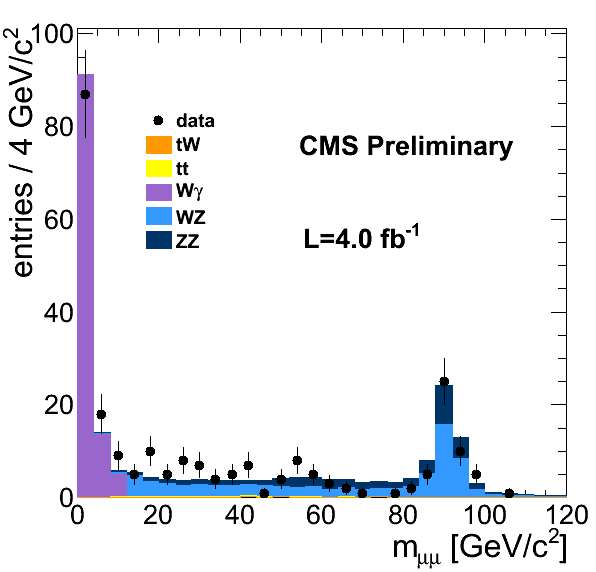
\includegraphics[width=0.5\linewidth]{figures/WGammaStar_mass_wholeSpectrum.png} 
\caption{\label{fig:WgammaStarMass}\protect Comparision of data and Monte Carlo for  
mass distributions of the muon pair associated with the virutal photon. 
All the selections defining the \Wgstar control region are applied but \ensuremath{M_{\mu\mu}<12} GeV.}
\end{center}
\end{figure}

To verify that the data belonging to the our control region have the expected features predicted
by the Monte Carlo we is suitable to describe the 



\begin{figure}[hbt]
\begin{center}
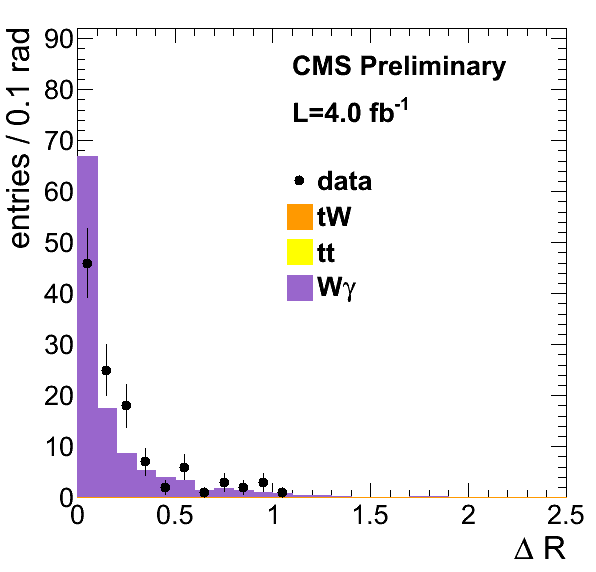
\includegraphics[width=0.3\linewidth]{figures/WGammaStar_dR.png} 
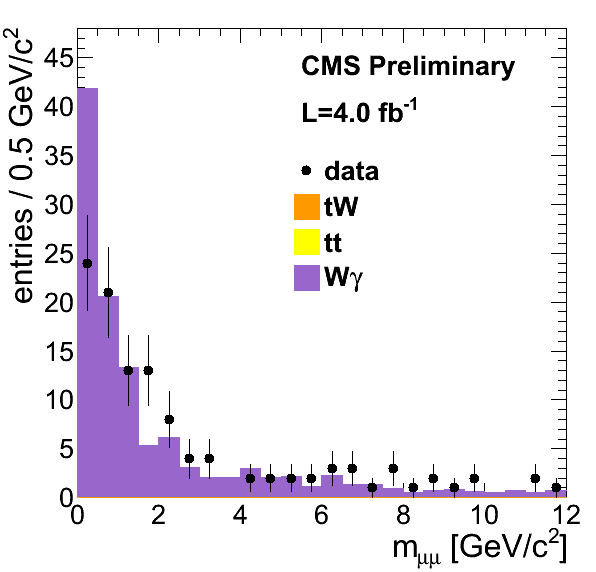
\includegraphics[width=0.3\linewidth]{figures/WGammaStar_mass.png}
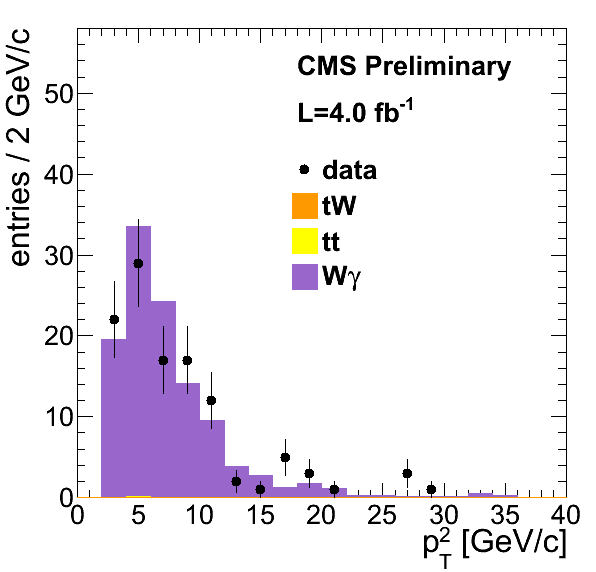
\includegraphics[width=0.3\linewidth]{figures/WGammaStar_3rdLep.png}
\caption{\label{fig:WgammaStar}\protect Comparision of data and Monte Carlo for three 
main distributions of the muons associated with the virutal photon in the \Wgstar control region. 
Left: opening angle (\delR).
Center: di-muon mass.
Right:. softest muon \pt.}
\end{center}
\end{figure}



